\subsection{Sistemas de detección de formaciones ferroviarias}
    \label{sec:detectors}
    
    Es de vital importancia que el sistema pueda determinar la posición de un tren dentro del tendido ferroviario. De esta manera, poder habilitar la circulación en secciones donde no exista peligro de colisión con otros formaciones o, por el contrario, detener la marcha de las formaciones anteriores para evitar accidentes. Existen diversas maneras de detectar la posición de un tren, entre ellas el uso de circuitos de vía y contadores de ejes(Figure \ref{fig:deteccion_1}). 

    \begin{figure}[!h]
        \centering
        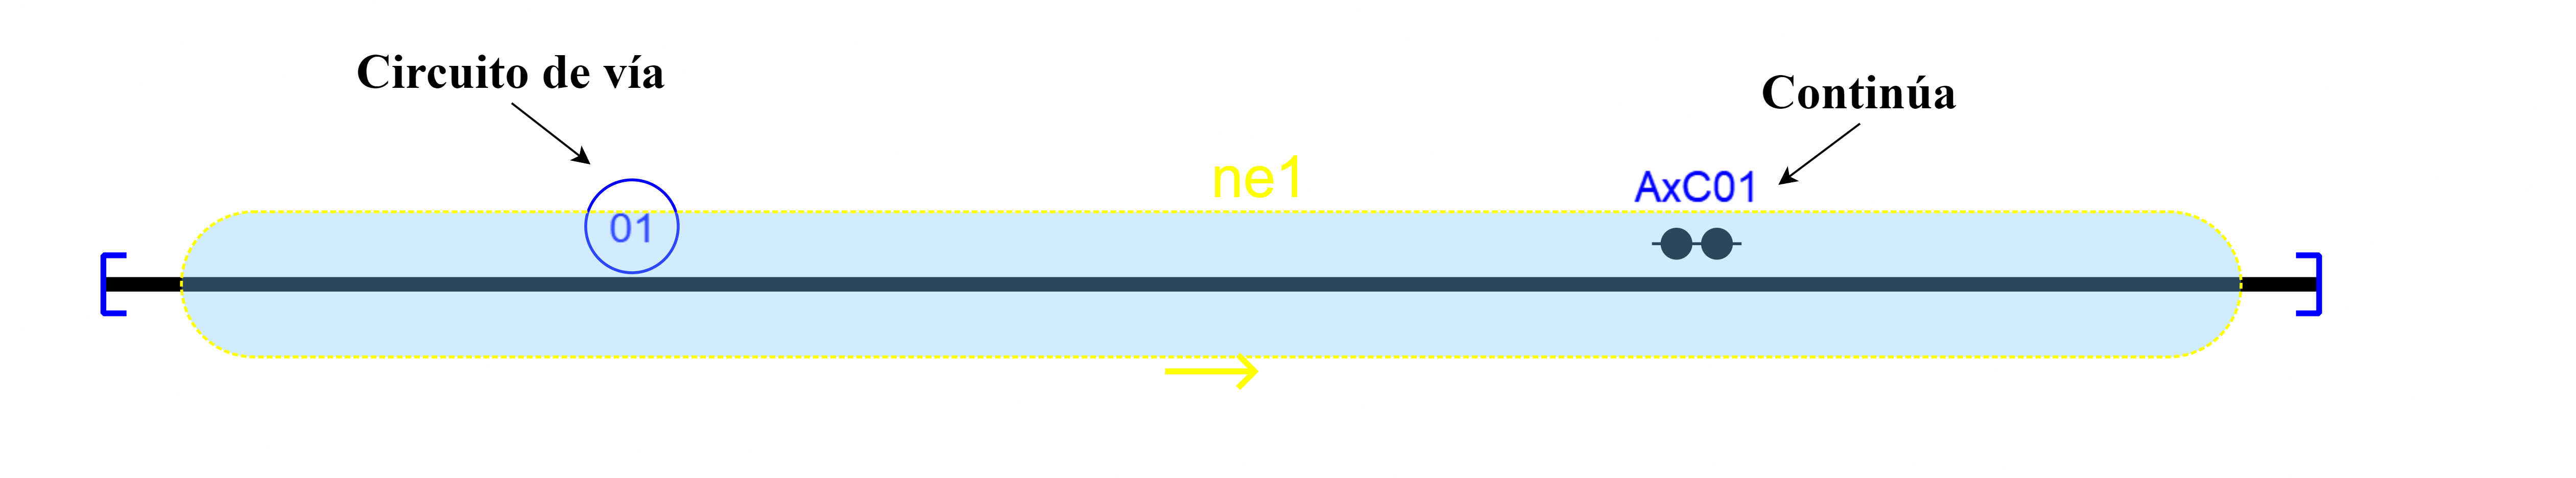
\includegraphics[width=1\textwidth]{Figuras/Detector.png}
        \centering\caption{Circuito de vía (04) y contador de ejes (AxC01).}
        \label{fig:deteccion_1}
    \end{figure}

    Los circuitos de vía (Figura \ref{fig:deteccion_2}) son dispositivos electrónicos que aplican una diferencia de potencial finita entre los rieles. Cuando una formación ingresa a la sección, sus ruedas metálicas cortocircuitan ambos rieles. El cortocircuito es detectado por el relé y este, a su vez, reporta el estado al resto del sistema. 

    \begin{figure}[!h]
        \centering
        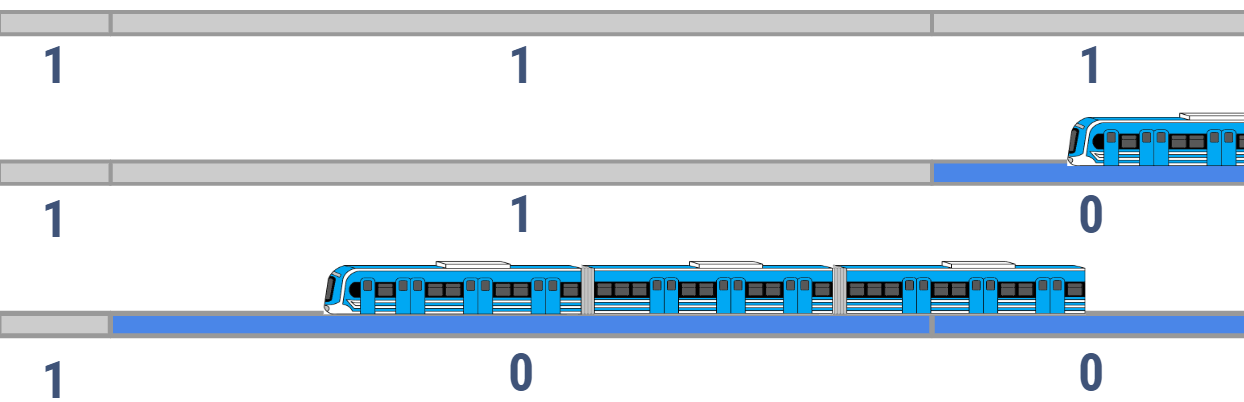
\includegraphics[width=1\textwidth]{Figuras/circuito_via}
        \centering\caption{Circuito de vía libre y ocupado.}
        \label{fig:deteccion_2}
    \end{figure}

    En caso de que la alimentación se interrumpa, el cableado sufra alguna falla, vandalismo, inundación, o que efectivamente una formación ocupe la sección, el circuito de vía reportará que la sección se encuentra ocupada. De esta manera, solo es posible recibir un reporte de sección desocupada cuando la sección efectivamente se encuentre desocupada. A este principio se le denomina fail-safe [REF]. Es decir, si por alguna razón algo falla, el sistema adopta la condición más restrictiva, mitigando la posibilidad de una situación peligrosa. 
    
    Existe una discontinuidad entre los rieles denominado juntura, que permite la expansión de los mismos al ser sometidos a altas temperaturas sin que los rieles se doblen y provoquen daños a la infraestructura. Los circuitos de vía, se relacionan directamente a las junturas entre las vías, modelados por la clase rail Joint en railML.  Esta discontinuidad eléctrica es lo que limita la acción del circuito de vía a la región entre dos junturas.

    En el código \ref{lst:trackCircuit} podemos ver un ejemplo de la clase tvdSection dentro de la clase interlocking, que incluye a la clase assetsForIL y estos, a su vez, a la clase vector de tvdSections. Esta clase posee un id (tvd7), la tecnología utilizada (en este caso trackCircuit, circuivo de vía) y los límites donde el circuito de vía es válido: los bufferStop bus1 y bus2.

    \begin{lstlisting}[language = XML, caption = Clase trackCircuit , label = {lst:trackCircuit}]
    <tvdSection id="tvd7" partialRouteReleaseDelay="PT4S" residualRouteCancellationDelay="PT90S" technology="trackCircuit" isBerthingTrack="false">
        <designator register="_Example" entry="04"/>
        <hasDemarcatingBufferstop ref="bus2"/>
        <hasDemarcatingBufferstop ref="bus1"/>
    </tvdSection>
    \end{lstlisting}

    Los sistemas contadores de ejes (Figura \ref{fig:deteccion_2}) consisten en sensores pasivos instalados en la cara interna de unos de los rieles y un sistema externo de procesamiento de datos. Estos sistemas no dependen de la aplicación de tensiones en la vía. Además, no solo permiten detectar la presencia de una formación, sino que también pueden usarse para medir la integridad de la formación, si se conoce a priori la cantidad de ejes de la misma. 

    \begin{figure}[!h]
        \centering
        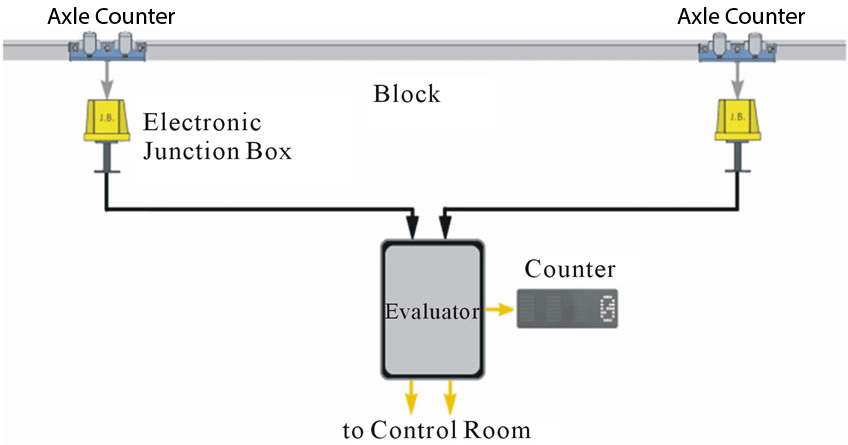
\includegraphics[width=1\textwidth]{Figuras/contador.jpg}
        \centering\caption{Contadores de ejes.}
        \label{fig:deteccion_2}
    \end{figure}

    Al igual que los circuitos de vía, los sistemas contadores de eje siguen el principio de fail-safe, adoptando la condición mas restrictiva en caso de falla. Ambos sistemas pueden utilizarse en simultáneo, de ser requerido. En el código \ref{lst:axleCounter} podemos ver un ejemplo de la clase trainDetectionElement, dentro de la clase functionalInfrastructure, dentro de la clase infrastructure. En este ejemplo la bclase fue definida como tipo axleCounter (contador de eje) y se le asigna el nombre AxC01 que vemos en la Figura \ref{fig:deteccion_1}, referido al netElement ne1. También podemos ver que este contador de ejes se activa en ambos sentidos (applicationDirection = both) y su coordenada intrínseca dentro del netElement ne1, dentro de los dos tercios de la sección.

    \begin{lstlisting}[language = XML, caption = Clase trainDetectionElement , label = {lst:axleCounter}]
    <trainDetectionElement id="ac6" type="axleCounter">
        <name name="AxC01" language="en"/>
        <spotLocation id="ac6_sloc01" netElementRef="ne1" applicationDirection="both" intrinsicCoord="0.6710"/>
        <designator register="_Example" entry="TRAIN DETECTION ELEMENT AxC01"/>
    </trainDetectionElement>
    \end{lstlisting}